% Appendix A
\label{AppendixA}
\chapter{Manuel d'utilisation - Commission de programme}
Ce manuel présente les différentes fonctionnalités qui sont offertes à la commission de programme. Tout au long de ce document il sera expliqué ou et comment se gère les catalogues de cours et les programmes de cours dans l'application. De plus, les conventions utilisées pour générer des graphes yEd et des formulaires Excel seront expliquées. 
\section{Gestion des catalogues de cours}


\subsection{Création d'un catalogue de cours}
\subsection{Mise à jour des informations contenues dans le catalogue de cours}
\section{Gestion des programmes des étudiants}

\begin{figure}
\centering

\includegraphics[width=\textwidth]{landing_page_access_to_catalog}
\caption{Accès de gestion des catalogues}
\label{fig:landing_page_catalog}
\end{figure}

Sur l'image ~\ref{fig:landing_page_catalog} apparaît la page d'accueil. Le menu pour accéder aux différents catalogues de cours est entouré d'un cadre rouge sur la capture d'écran. Les menus entourés du cadre bleu donnent accès aux différentes fonctionnalités offertes pour gérer les programmes des étudiants. Nous y reviendrons plus tard. 

\subsection{Accéder aux catalogues}
Après avoir cliquer sur le menu catalogue, nous arrivons sur la page montrant les différents cours présents dans l'application. Comme vous pouvez le voir sur la capture d'écran ~\ref{fig:catalog_index}, il n'y a qu'un seul catalogue pour le moment dans l'application. Vous pouvez cliquer sur la petite loupe en dessous de la colonne nommée \textit{info} pour accéder au catalogue en question ou sur la petite croix \textcolor{red}{rouge} pour le supprimer de l'application.

La section qui suit va expliquer les conventions à respecter lorsque l'on crée un graphe de cours avec yEd.

\begin{figure}
\centering
\caption{Liste des catalogues}
\label{fig:catalog_index}
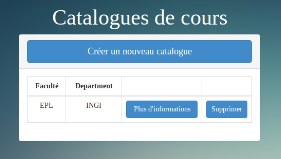
\includegraphics[width=\textwidth]{catalog_index}
\end{figure}

\subsection{Construction d'un catalogue de cours avec yEd}
Dans cette section nous allons pas à pas construire un graph de cours avec yEd (l'outil utilisé pour générer des graphes de cours).

Yed est disponnible ici \url{http://www.yworks.com/en/downloads.html\#yEd}

Nous allons créé un  catalogue de cours fictif, composé d'un programme, d'un module, de quelques cours et de quelques dépendances. Tout d'abord, ouvrez le programme yEd et créer un nouveau document. Une fois le yEd ouvert et le nouveau graph créer, vous verrez à votre droite le menu suivant ~\ref{fig:yed_menu}.

\begin{figure}[!htb]
\centering
\caption{Menu de yEd}
\label{fig:yed_menu}
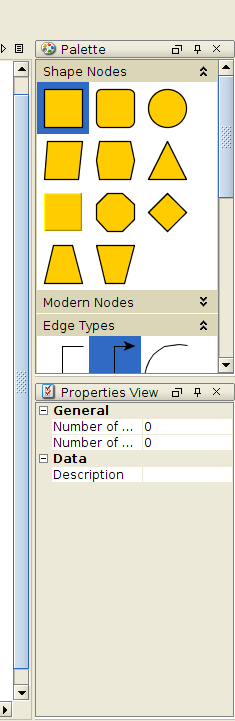
\includegraphics[scale=0.5]{yed_menu}
\end{figure}


\subsubsection{Créer des cours}
Pour créer les objets représentant les cours, il faut utiliser ce menu ~\ref{fig:yed_node_menu} et sélectionner le carré (en \textcolor{blue}{bleu sur la capture d'écran}) puis cliquer sur le document pour l'ajouter au graphe.

\begin{figure}
\centering
\caption{Menu de création des noeuds}
\label{fig:yed_node_menu}
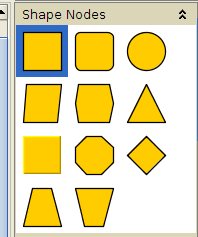
\includegraphics[scale=0.6]{yed_node_menu}
\end{figure}

Pour nommer le nœud:
\begin{enumerate}
\item Clique droit sur le nœud
\item Cliquez sur \textit{properties}
\end{enumerate}

Le menu suivant apparaîtra ~\ref{fig:properties_menu}. Il suffit de remplir le champ \textit{Texte} avec le nom désiré.

\begin{figure}
\centering
\caption{Ajouter un nom à un noeud}
\label{fig:properties_menu}
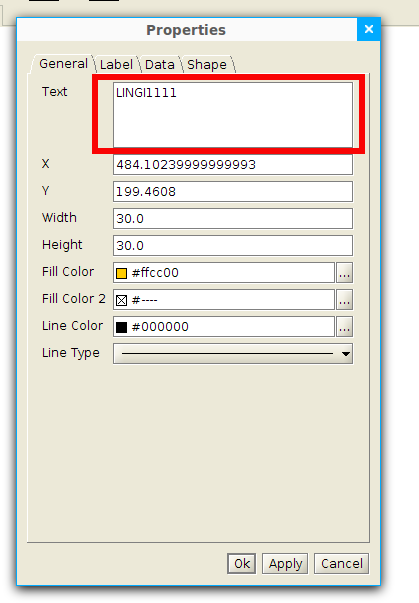
\includegraphics[scale=0.6]{properties_menu}
\end{figure}


\subsubsection{Ajouter des dépendances}

Pour représenter les dépendances entre les cours, il faut utiliser le menu présent sur l'image  ~\ref{fig:yed_edge_menu} qui permet de dessiner des arrêtes entre les nœuds.

\begin{figure}
\centering
\caption{Menu de création d’arêtes}
\label{fig:yed_edge_menu}
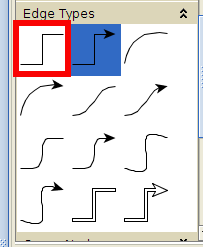
\includegraphics[scale=0.6]{yed_edge_menu}
\end{figure}

Nous utilisons deux type d’arêtes;

\begin{itemize}
\item en \textcolor{blue}{bleu} sur l'image ~\ref{fig:yed_edge_menu}, les arrêtes pour représenter les prérequis
\item en \textcolor{red}{rouge} sur l'image ~\ref{fig:yed_edge_menu}, les arrêtes pour représenter les corequis
\end{itemize}

Pour représenter les dépendances n-aire, l'application reconnait la convention suivante:

Simplement sélectionner un losange ou un rond, mettre le label \textbf{X pour représenter une contrainte disjonctive excusive (XOR)} ou {OR pour représenter une contrainte disjonctive (OR)} et la connecter aux différents cours concernés avec la contrainte (prérequis ou corequis) correspondante.

\begin{itemize}
\item Sur l'image \ref{fig:or_depandancy} est illustré à quoi doit ressembler une contrainte n-aire disjonctive.
\item Sur l'image \ref{fig:xor_depandancy} est illustré à quoi doit ressembler une contrainte n-aire disjonctive exclusive.
\end{itemize}

En créant un catalogue de deux cours, avec l'un étant le prérequis de l'autre, nous obtenons le graph présent sur l'image suivante ~\ref{fig:dependancies_example}.

\begin{figure}[!htb]
\centering
\caption{Prérequis n-aire disjonctif}
\label{fig:or_depandancy}
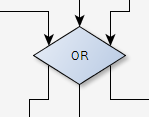
\includegraphics[scale = 1]{OR_dependancie}
\end{figure}

\begin{figure}[!htb]
\centering
\caption{Prérequis n-aire disjonctif exclusif}
\label{fig:xor_depandancy}
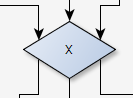
\includegraphics[scale = 1]{XOR_dependancie}
\end{figure}

\begin{figure}[!htb]
\label{fig:dependancies_example}
\centering
\caption{Deux cours avec une dépendance}
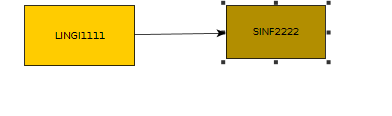
\includegraphics[scale=0.5]{dependancies_example}

\end{figure}

\subsubsection{Insérer des cours dans des modules}
Après avoir créer plusieurs cours, il est possible de regrouper ces nœuds dans une boite.
\begin{enumerate}
\item Sélectionner les noeuds à regrouper
\item Clique droit
\item Cliquer sur \textit{grouping}
\end{enumerate}

Vous obtiendrez une boite comme sur la capture ~\ref{fig:node_grouping}

\begin{figure}
\centering
\caption{Mettre des nœuds dans une boite}
\label{fig:node_grouping}
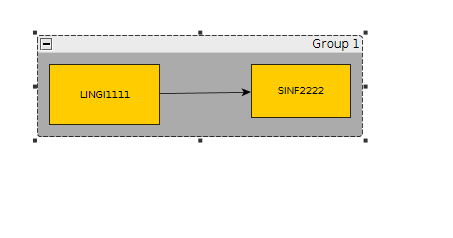
\includegraphics[scale=0.5]{node_grouping}
\end{figure}

La démarche à suivre pour nommer les boites est la même que celle pour nommer les nœuds.

Avant de poursuivre, il est nécessaire de préciser la structure de graph reconnue par l'application. 

\begin{itemize}
\item Un \textbf{catalogue} est représenté par un \textbf{graphe} et est composé exclusivement de \textbf{programmes}
\item Un \textbf{programme} est représenté par une \textbf{boite} et est composé de \textbf{modules} et de \textbf{cours}
\item Un \textbf{module} est représenté par une \textbf{boite} et est composé de plusieurs \textbf{sous-modules} et \textbf{cours}
\item Un \textbf{sous-module} marquera dans l'application tout les \textbf{cours} qu'il contient comme obligatoire pour le \textbf{module} parent.
\item Un \textbf{cours} est représenté par un \textbf{nœud} et peut avoir plusieurs dépendances. 
\item Une \textbf{dépendance} est représenté par une \textbf{arrête} entre deux \textbf{nœuds}.(Elle peut avoir deux type comme expliqué plus tôt
\end{itemize}

Sur l'image \ref{fig:small_catalog_example}, vous pouvez voir un exemple de catalogue valide.

\begin{figure}
\centering
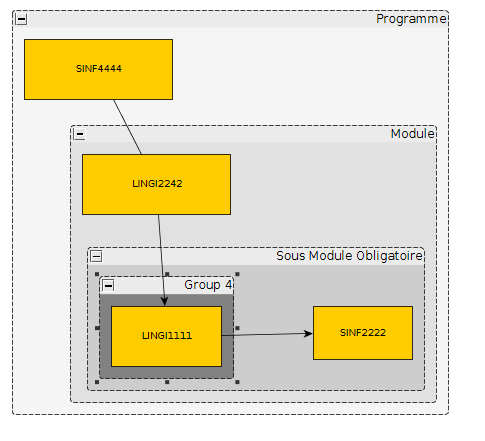
\includegraphics[scale=0.6]{small_catalog_example}
\label{fig:small_catalog_example}
\caption{Un (petit) catalogue de cours valide}

\end{figure}

%*************************************************


\subsection{Création d'un catalogue - Import du graph dans l'application}
Une fois le graphe créé avec yEd, il ne reste plus qu'à créer un nouveau catalogue de cours en important ce graphe dans l'application. Depuis la page illustrée sur la capture d'écran \ref{fig:catalog_index}, cliquez sur \textbf{Créer un nouveau catalogue}.

Le formulaire qui permet de créer un nouveau catalogue est illustré sur la capture suivante \ref{fig:catalog_new}.

\begin{figure}
\centering
\caption{Création d'un catalogue de cours}
\label{fig:catalog_new}
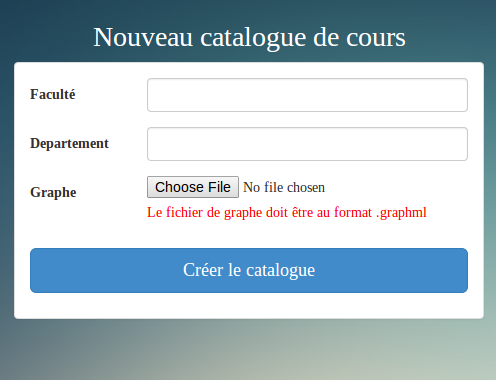
\includegraphics[scale=0.6]{catalog_new}
\end{figure}

Remplissez, les champs (qui identifient votre catalogue), sélectionner le fichier de graph désiré et cliquez sur \textit{Créer le catalogue}

Vous arrivez sur la page présentée sur l'image suivante \ref{fig:catalog_show_manual}. Le bouton \textbf{Télécharger le fichier excel} permet de récupérer sous forme de formulaire excel les informations, à propos du catalogue de cours, qui sont contenues dans la base de données. Le bouton \textbf{Mettre à jour les informations} permet, quant à lui, de mettre à jour ces données avec le fichier Excel sélectionné avec me menu \textbf{choose file}.

\begin{figure}
\centering
\caption{Le catalogue une fois créé}
\label{fig:catalog_show_manual}
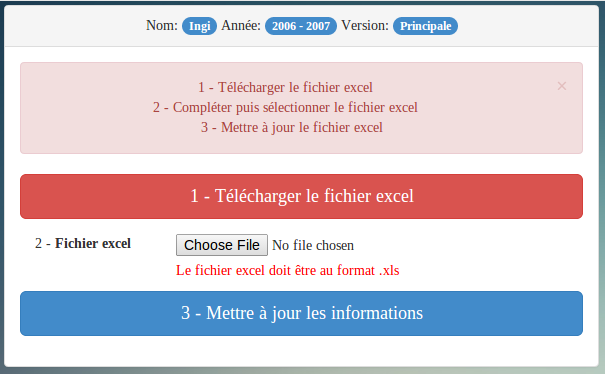
\includegraphics[width = \textwidth]{catalog_show_manual}
\end{figure}

\subsection{Mise à jour des informations contenues dans le catalogue}
Les informations contenue dans le graphe yEd n'étant pas complète, il est nécessaire, après avoir créer le catalogue, de compléter ses informations à l'aide d'un formulaire excel. Cette sous-section va expliquer les conventions à utiliser pour cela.

 


Pour ce faire il est conseillé  de \textbf{commencer par télécharger le formulaire Excel} (en cliquant sur le bouton en \textcolor{red}{rouge} sur l'image \ref{fig:catalog_show_manual}) contenant les informations du catalogue, les pages correctement nommées, ainsi que certaines proposition d'attributs à ajouter au catalogue. Il est préférable de ne pas passer cette étape. Dans le cas contraire, vous serez obligé d'écrire les identifiants de tout les différents programmes, modules et cours un à un dans le formulaire. Pour un catalogue de 55 cours, cela peut être long. 

Le formulaire est structuré comme suit:
\begin{itemize}
\item une page par objet cours, modules et programme;
\item la page relative au programme doit être nommée \textbf{PROGRAMMES};
\item la page relative au cours doit être nommée \textbf{COURS};
\item la page relative au modules doit être nommée \textbf{MODULES};
\item chaque colonne d'une page correspond à la propriété de l'objet en question;
\item le premier élément de chaque colonne (en \textbf{gras}) identifie le nom de la propriété (SIGLE pour la colonne relative aux sigles d'un cours par exemple);
\item les éléments sont identifiés en fonction de leur ligne dans le formulaire; le module d'import va chercher la colonne intitulé NAME (ou SIGLE si c'est un cours);
\item pour chaque élément de la colonne NAME (ou SIGLE), le module va rechercher l'objet qui est identifié par cette propriété, puis va ajouter un à un toute les propriétés se trouvant sur la même ligne que cet élément. 
\end{itemize}

Cette étape est répétable à l’infini. Ce pendant, faites attention à la cohérence des informations mises dans ce document. Le module d'import de fichiers Excel ne les détecte pas encore les incohérences qui peuvent y survenir. 

Remarques:
\begin{itemize}
\item il faut remplir coute que coute la colonne \textbf{SEMESTRE} de la page \textbf{COURSES} identifiant le semestre durant le quel est dispensé un cours (si cette propriété n'est pas définie, ils ne seront pas affichés aux étudiants);
\item attention à ne pas se tromper en utilisant les propriétés concernant les minimum et maximum de crédits d'un module ou d'un programme; un exemple d'incohérence serait un programme dont le maximum de crédits autorisés serait inférieur à la somme des minimum de crédits autorisés des modules qui le compose.
\end{itemize}



Une fois le \textit{template} de formulaire téléchargé et complété , sélectionnez le et cliquez sur le bouton \textit{Mettre à jour les informations} (en \textcolor{blue}{bleu} sur l'image \ref{fig:catalog_show_manual}).


Un message en \textcolor{blue}{bleu} vous avertira du succès de l'opération.


\subsection{Naviguer à travers les programmes de cours}

Pour inspecter les différents programmes ainsi que les modules et les cours qui le compose descendez sur la page \ref{fig:programs_index} et cliquez sur les différents onglets pour naviguer à travers les différents programmes, modules et cours. Tout cela se déroule sans devoir recharger la page. Pour obtenir encore plus d'information sur un cours, programme ou module, il suffit de cliquer sur la petite loupe en \textcolor{blue}{bleu}. Pour supprimer un élément, cliquez sur la croix \textcolor{red}{rouge}

\begin{figure}
\centering
\caption{Programmes, modules et cours}
\label{fig:programs_index}
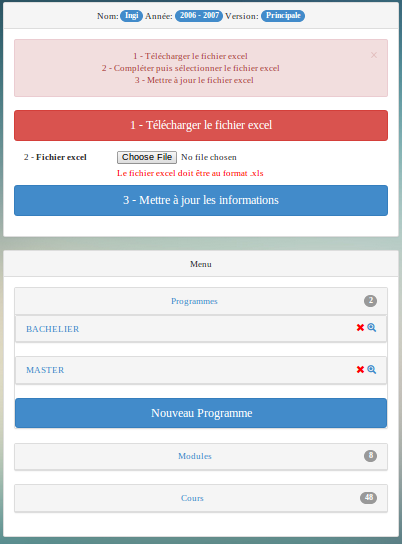
\includegraphics[width = \textwidth]{programs_index}

\end{figure}



\section{Gestion des demandes de validations}
Lorsqu'un étudiant désire envoyer le programme qu'il s'est créé à la validation, une demande de validation est envoyé à la \textbf{commission INFO}. Pour accéder à ces demandes de validations, 
il suffit de cliquer sur le menu intitulé \textit{Validations} entouré en rouge sur l'image \ref{fig:landing_page_catalog}.

Sur la page des validations (Image~\ref{fig:validations}) vous pouvez:
\begin{itemize}
\item inspecter le programme que l'étudiant demande de valider en cliquant sur la petite loupe en \textcolor{blue}{bleu} (en dessous du menu \textbf{Programme});
\item accéder à la justification de l'étudiant en cliquant sur la petite loupe en \textcolor{blue}{bleu} (en dessous du menu \textbf{Justification});
\item valider la requête en cliquant sur \textit{Valider} (en \textcolor{green}{vert} sur l'image \ref{fig:validations});
\item refuser la requête en cliquant sur \textit{Refuser} (en \textcolor{red}{rouge} sur l'image \ref{fig:validations}).
\end{itemize}

\begin{figure}
\centering
\caption{Gestion des demandes de validations}
\label{fig:validations}
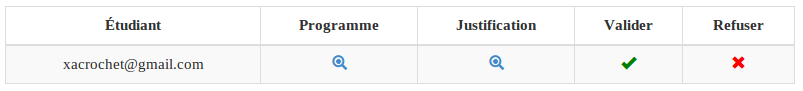
\includegraphics[scale=0.6]{validations}
\end{figure}
\subsection{Justification d'un étudiant}
Lorsque vous accéder au menu justification, vous arrivez sur la page illustrée sur la capture d'écran \ref{fig:justification_example}

\begin{figure}
\centering
\caption{Exemple de justification}
\label{fig:justification_example}
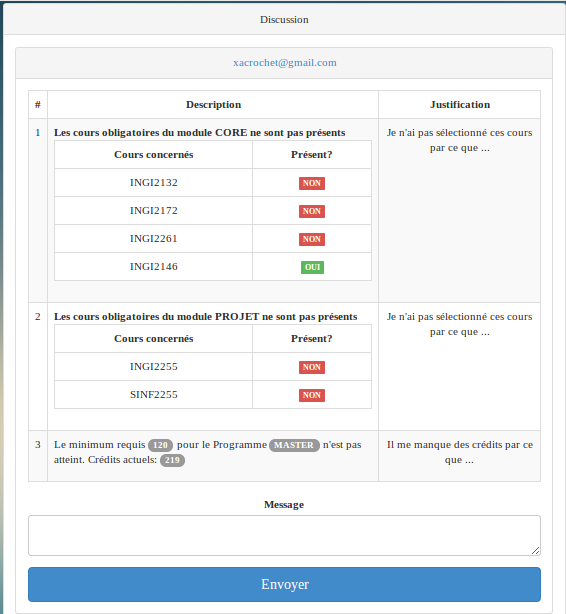
\includegraphics[width=\textwidth]{justification_example}
\end{figure}

Dans la colonne de gauche (\textbf{Description}) s'affiche toutes les contraintes non-respectée du programme de l'étudiant. 

Dans la colonne de droite (\textbf{Justification})s'affiche chacune des justifications de l'étudiant.

Tout en bas, un message peut être envoyé à l'étudiant, pour lui demander des informations supplémentaires par exemple. 

Le menu discussion de la page \ref{fig:landing_page_catalog} (dans les menus entourés d'un cadre \textcolor{blue}{bleu}) permet d'accéder directement à toute les justifications des étudiants.

\section{Gestion des années}

En cliquant sur le menu \textbf{Gérer les années} de la page \ref{fig:landing_page_catalog}, on accède à la page \ref{fig:manage_years} qui permet de gérer les années des étudiants. C'est ici que l'on peut marquer une année comme ratée ou réussie. 

Il est important de marquer les années après chaque année académique. Le statut des anciennes années est utilisé pour vérifier la validités des dépendances de cours. En effet, un prérequis dont le cours, présent dans une année ratée, n'a pas été crédité ne sera pas valide. 

\begin{figure}
\centering
\caption{Gérer les années des étudiants}
\label{fig:manage_years}
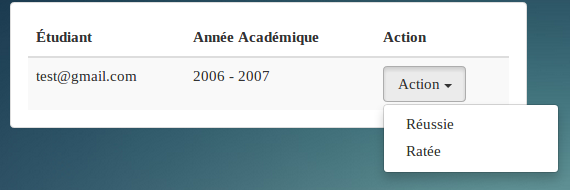
\includegraphics[width=\textwidth]{year_mgmt}
\end{figure}

Pour marquer une année comme réussie, il suffit de sélectionner l'action nommée \textbf{Réussie}. L'année et ses cours seront ainsi crédités. 

Lorsque l'on marque une année comme ratée, on arrive sur la page \ref{fig:fail_year}. Sur cette page, il faut sélectionner les cours qui ont été crédités.

\begin{figure}
\centering
\caption{Marquer une année comme ratée}
\label{fig:fail_year}
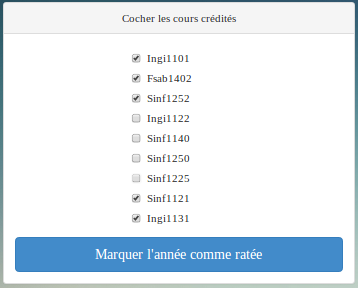
\includegraphics[width=\textwidth]{failed_year_mgmt}

\end{figure}


